\section{Introdução}

\subsection{Motivação}

\begin{frame}

  \begin{minipage}[c]{0.8\linewidth}
    \begin{center}
      \it Se uma imagem vale mais que 1000 palavras então\ldots
      \pause~\\
      um recurso interativo vale mais que 1000 imagens.
    \end{center}
  \end{minipage}
  \vspace{2em}

  \begin{multicols}{2}
    \pause
    \begin{block}{Objetivo}
      Apresentar ferramentas para facilitar
      \begin{enumerate}
        \itemsep-2pt\parskip0pt\parsep0pt
      \item a compreensão de conceitos/resultados,
      \item a realização de tarefas e
      \item como compartilhar esses recursos.
      \end{enumerate}
    \end{block}
    \vfill \columnbreak \pause
    \begin{block}{Uso em potencial}
      \begin{itemize}
      \item como instrumento de ensino,
      \item para construir mini aplicativos e
      \item para produzir relatórios/aplicações web interativos.
      \end{itemize}
    \end{block}
  \end{multicols}
\end{frame}

\begin{frame}
  Nossa experiência
  \begin{multicols}{2}
    \begin{itemize}
    \item Animações para matérias de blog;
    \item Instrumento de ensino em material online;
    \item Aplicação para ajuste de modelos não lineares;
    \item Aplicações para ensino de Estatística;
    \end{itemize}
    \vfill \columnbreak
    \begin{itemize}
    \item O Grupo PET Estatística desenvolveu várias aplicações para
      feira de profissões;
    \item Discentes criam a Academia de Estatística Computacional e
      Programação;
    \item Aquisição da servidora RStudio/Shiny do LEG \& PET;
    \item Crescente demanda de recursos para visualização de dados
      espaço temporais.
    \end{itemize}
  \end{multicols}
\end{frame}

\subsection{Conteúdo}

\begin{frame}
  \vspace{-1.0cm}
  \begin{columns}[t]
    \begin{column}{.3\textwidth}
      \vspace{1cm}
      \begin{block}{Recursos interativos}
        \begin{itemize}
          \setbeamercovered{transparent=35} \uncover<2>{\item
            \texttt{animation}} \uncover<3>{\item \texttt{rgl}}
          \uncover<4>{\item \texttt{googleVis}} \uncover<5>{\item
            \texttt{gWidgets}} \uncover<6>{\item \texttt{rpanel}}
          \uncover<7>{\item \texttt{shiny}}
        \end{itemize}
      \end{block}
      \vspace{1cm}
    \end{column}
    \begin{column}{.6\textwidth}
      \vspace{0.5cm} \only<2>{ {\center
          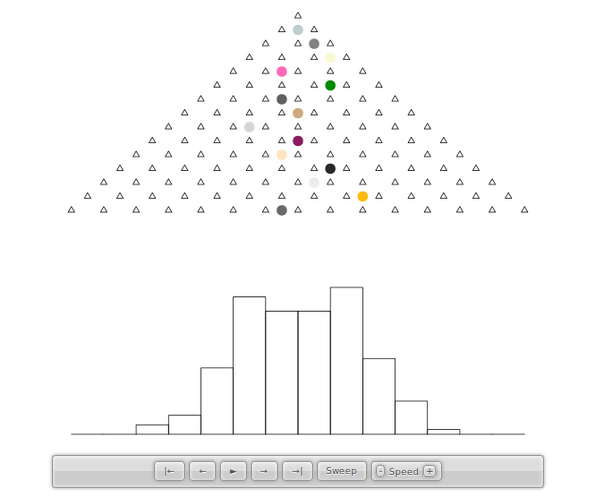
\includegraphics[scale=0.3]{images/preview_ani}}} \only<3>{
        {\center
          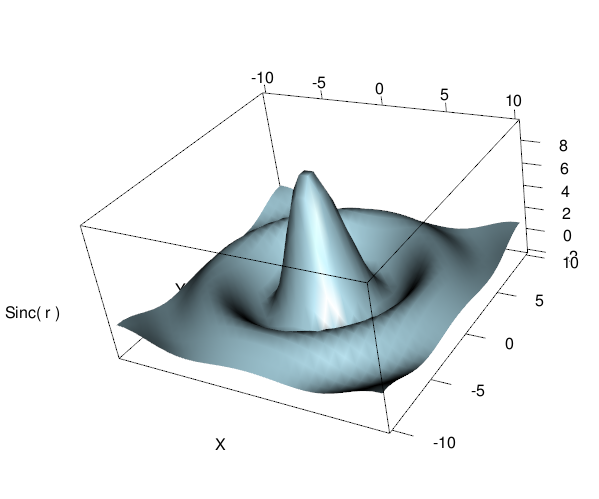
\includegraphics[scale=0.3]{images/preview_rgl}}} \only<4>{
        {\center \vspace{-0.7cm}
          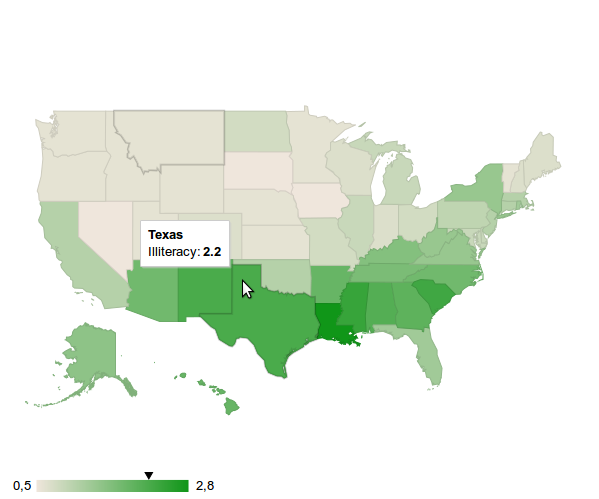
\includegraphics[scale=0.3]{images/preview_ggvis}}} \only<5>{
        {\center
          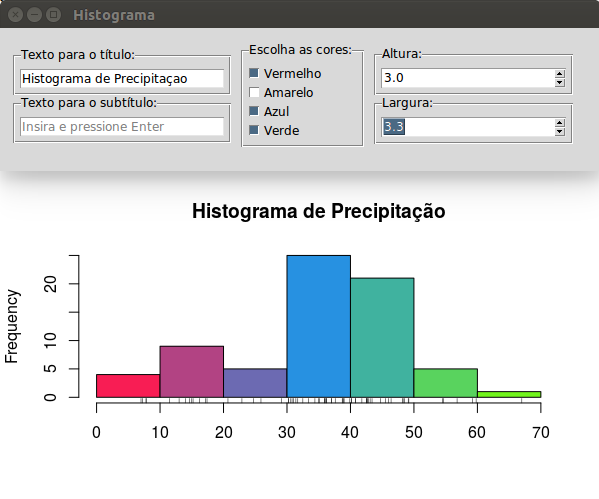
\includegraphics[scale=0.3]{images/preview_gwidgets}}}
      \only<6>{ {\center
          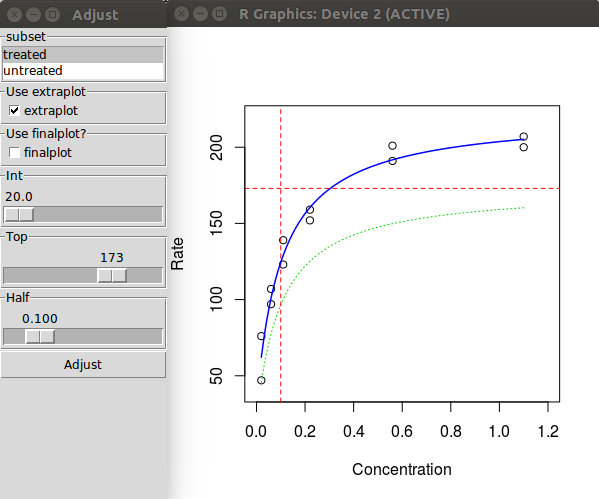
\includegraphics[scale=0.3]{images/preview_rpanel}}} \only<7>{
        {\center
          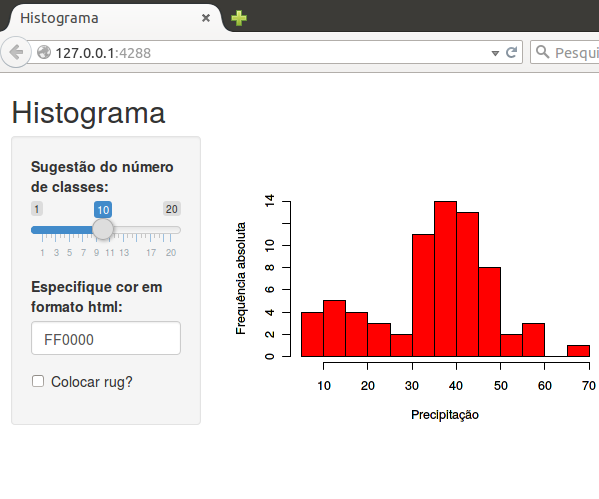
\includegraphics[scale=0.3]{images/preview_shiny}}}
    \end{column}
  \end{columns}
\end{frame}
